% arara: pdflatex: { synctex: yes }
% arara: makeindex: { style: ctuthesis }
%% arara: bibtex

%\listfiles


%\PassOptionsToPackage{cp1250}{inputenc}

% The class takes all the key=value arguments that \ctusetup does,
% and couple more: draft and oneside
\documentclass[oneside]{ctuthesis}

% MY IMPORTS
\usepackage{pdfpages}

\makeatletter
\edef\mytoday{\expandafter\@gobbletwo\the\year\ifnum\month<10 0\fi\the\month\ifnum\day<10 0\fi\the\day}
\makeatother

% LaTeX logo with better kerning in sf bf font
\makeatletter
\newcommand\LaTeX@lmss@bx{L\kern -.33em{\sbox \z@ T\vbox to\ht \z@ {\hbox {\check@mathfonts \fontsize \sf@size \z@ \math@fontsfalse \selectfont A}\vss }}\kern -.15em\TeX}
\DeclareRobustCommand\myLaTeX{%
	\ifcsname LaTeX@\f@family @\f@series\endcsname
		\csname LaTeX@\f@family @\f@series\endcsname
	\else
		\LaTeX
	\fi
}


\ctusetup{
	mainlanguage = english,
	secondlanguage = czech,
	otherlanguages = {czech},
%   title-czech = {Bias Detection in Czech News},
	title-english = {Bias Detection in Czech News},
	doctype = B,
	faculty = F3,
	department-czech = {Katedra počítačů},
	department-english = {Department of Computer Science},
	author = {Tomáš Horych},
	supervisor = {Ing. Jan Drchal, Ph.D},
	fieldofstudy-english = {Open Informatics},
	subfieldofstudy-english = {Artificial Intelligence and Computer Science},
	fieldofstudy-czech = {Matematcké inženýrství},
	subfieldofstudy-czech = {Matematické modelování},
	keywords-czech = {zpracování přirozeného jazyka, detekce zaujatosti, mediální bias, detekce subjektivity, klasifikace textu},
	keywords-english = {natural language processing, bias detection, media bias,subjectivity detection, text classification},
	day = 10,
	month = 2,
	year = 2022,
	specification-file = {my_modules/assignment.pdf},
	front-specification = true,
    pkg-listings = true,
    ctulstbg = none,
}

\ctuprocess

% Theorem declarations, this is the reasonable default, anybody can do what they wish.
% If you prefer theorems in italics rather than slanted, use \theoremstyle{plainit}
\theoremstyle{plain}
\newtheorem{theorem}{Theorem}[chapter]
\newtheorem{corollary}[theorem]{Corollary}
\newtheorem{lemma}[theorem]{Lemma}
\newtheorem{proposition}[theorem]{Proposition}

\theoremstyle{definition}
\newtheorem{definition}[theorem]{Definition}
\newtheorem{example}[theorem]{Example}
\newtheorem{conjecture}[theorem]{Conjecture}

\theoremstyle{note}
\newtheorem*{remark*}{Remark}
\newtheorem{remark}[theorem]{Remark}

% Marginpars used as navigation aids.
\usepackage{mparhack}
\usepackage{hyperref}
\usepackage[autostyle]{csquotes} 
\usepackage{subfig}

% glossary input
\usepackage{glossaries}

\makeglossaries
\newacronym{nup}{NÚP}{\textit{Nezaujatý Úhel Pohledu}}
\newacronym{iaa}{IAA}{Inter-Annotator Agreement}
\newacronym{mbg}{MBG}{Media Bias Group}
\newacronym{npov}{NPOV}{Neutral~Point~Of~View}
\newacronym{wnc}{WNC}{Wiki Neutrality Corpus}
\newacronym{nfnz}{NFNZ}{Nadační fond nezávislé žurnalistiky}
\newacronym{nmt}{NMT}{Neural Machine Translation}
\newacronym{nlp}{NLP}{Natural Language Processing}
\newacronym{ml}{ML}{Machine Learning}
\usepackage{colortbl}
\definecolor{unbiased_clr}{RGB}{183,235,198}
\definecolor{biased_clr}{RGB}{236,189,189}
\definecolor{biasedw_clr}{RGB}{225,130,130}

\newcommand\indexmp[1]{{\sffamily\bfseries#1}}

\ExplSyntaxOn
\cs_new:Nn \ctuman_domarginpar:n {
	\marginpar
	[ \raggedleft \footnotesize \sffamily #1 ]
	{ \raggedright \footnotesize \sffamily #1 }
}
\cs_generate_variant:Nn \ctuman_domarginpar:n { x }
\DeclareDocumentCommand \ctump { m } {
	\clist_set:Nn \ctuman_temp_clist { #1 }
	\ctuman_domarginpar:x { \clist_use:Nnnn \ctuman_temp_clist { \\ } { \\ } { \\ } }
	\clist_map_inline:Nn \ctuman_temp_clist { \index{##1|indexmp} }
	\ignorespaces
}
\ExplSyntaxOff



% Abstract in Czech
\begin{abstract-czech}
Automatická detekce zaujatosti v médiích představuje možnou cestu k objektivnějšímu a faktičtějšímu psaní. Tato práce se zaměřuje na zaujatost médií a zabývá se problémem binární klasifikace zaujatosti médií v českém zpravodajském prostředí. Je zde proveden přehled literatury a metodiky pro různé aspekty zaujatosti. Následně je shromážděn a analyzován soubor dat týkajících se zajuatosti médií. S využitím strojového překladu je prezentováno osm paralelních českých datasetů, přičemž jeden z nich je rozsáhlý dataset o 360 tisících větách. Kromě toho je z wikipedie automaticky extrahován nový český dataset CWNC (Czech Wiki Neutrality Corpus) pro detekci zaujatosti, s 5 766 větami. Následné experimenty pak ukazují vliv předtrénování na kombinacích aktuálních dostupných doménových datasetů a naznačují pozitivní vliv předtrénování na datasetech zaměřených na subjektivitu. Český BERT model s nejlepšími parametry a nastavením pak dosahuje skóre F1 \textbf{80,2\%} na vybraném testovacím dataset. Nakonec je natrénovaný klasifikátor využit ke klasifikaci reálných dat z různých zpravodajských zdrojů.

\end{abstract-czech}

% Abstract in English
\begin{abstract-english}
Automatic detection of bias in media represents a possible way to more objective and factual writing. This work focuses on \textbf{media bias} and adresses the problem of binary classification of media bias in the czech news environment. A literature and methodology for different aspects of bias is reviewed. Then a set of datasets related to media bias is collected and analyzed. Utilizing the machine translation, eight parallel czech datasets are presented with one being a large-scale dataset of 360k sentences. Additionally, a novel Czech dataset CWNC (Czech Wiki Neutrality Corpus) for bias detection with 5,766 sentences is automatically extracted from wikipedia. Following experiments then show effects of pre-training on combinations of current in-domain datasets, suggesting a positive effect of pre-training on subjective datasets. Czech BERT-based model with best parameters and setting then achieves F1 score of \textbf{80.2\%} on a selected target dataset. Finally a trained classifier is utilized to classify real-world data from various news sources.

\end{abstract-english}

% Acknowledgements / Podekovani
\begin{thanks}
I thank to my supervisor, Jan Drchal, for the guidance through the Machine Learning and NLP methodology and for supporting my research interests. I would also like to thank to my family, who always supported me during my studies and throughout the process of work on this thesis.
\end{thanks}

% Declaration / Prohlaseni
\begin{declaration}
I declare that the presented work
was developed independently and that
I have listed all sources of information
used within it in accordance with the
methodical instructions for observing
the ethical principles in the preparation
of university theses.

\medskip

In Prague, \monthinlanguage{title} \ctufield{day}, \ctufield{year}

\medskip

\end{declaration}

\usepackage{url}
\usepackage{subfig}

\usepackage{tabularx,array}
\usepackage{mathtools,amssymb}


% A savebox for typesetting listings in the titles
\newsavebox{\myboxa}

%\newcommand*\symbO{$\color{red}\bowtie$}
\newcommand*\symbO{\raisebox{0.5\height}{\scalebox{0.7}{\color{red}${\vartriangleright}\mkern-6mu{\vartriangleleft}$}}}
\newcommand*\symbM{\raisebox{0.5\height}{\scalebox{0.7}{\color{red}${\blacktriangleright}\mkern-6mu{\blacktriangleleft}$}}}
\newcommand*\itemO{\item\leavevmode\kern-0.33em\symbO}
\newcommand*\itemM{\item\leavevmode\kern-0.33em\symbM}


\begin{document}

% We actually don't want inline listings to have a background color
\renewcommand \ctulstsep {0pt}

% \ctuclsname for typesetting the class' name
\newcommand\ctuclsname{\leavevmode\unhcopy\ctuclsnamebox}
\newsavebox\ctuclsnamebox
\begin{lrbox}{\ctuclsnamebox}
\ctulst!ctuthesis!
\end{lrbox}

% all the formal stuff (abstract, title page etc)

\maketitle















%-------------------------------------------------------------------------------------------------------------------
% MAIN TEXT
\chapter{Introduction}
This is introduction to my thesis, motivation. taky něco o nlp
\section{Motivation}
tady něco o nlp
\section{Outline}



\chapter{Bias Detection}
Before turning my attention to media bias, I have examined several other relevant bias detection topics. At the beginning of my research, I studied the possibilities of applying gender bias detection to Czech News. Therefore, the following small section is dedicated to my results and examination of one of the gender-focused datasets.


%______________________________GENDER______________________________________________%
\section{Gender bias detection}\label{gender}
Most of the work on gender bias aims to study gender bias embedded in models and other methods to measure, clarify, and possibly mitigate it.

There is clear evidence that current language models possess implicit gender bias. Whether it means, in terms of learning biased embeddings \cite{bolukbasi2016man}, or simply underrepresentation of a particular gender in the data \cite{sun-peng-2021-men}. 

Yet, my work aspires to classify news texts; therefore, I examined the possibilities of gender classification in text.

I closely followed the approach of Dinan et al. \cite{dinan2020multi}. They define three dimensions of gender bias: bias when speaking \textit{ABOUT} someone, \textit{TO} someone or \textit{AS} someone. Target classes are \{masculine,feminine,neutral\}. 

The \textit{bias} here simply means an aspect of the statement that implies the gender of a particular person along the dimensions. To make this definition more clear, for example, the authors further propose that an unbiased sentence would be a sentence in which a machine learning model would not be able to classify a gender because there would basically be no difference between the classes. Yet, in a real-world scenario, sentences \textbf{are} influenced by gender, and therefore such classification is possible.

To measure this kind of bias over all three dimensions, a large-scale dataset \textbf{md\_gender}\footnote{\url{https://huggingface.co/datasets/md_gender_bias}} has been collected. The authors train a transformer model using \Gls{mtl}, to capture all three dimensions. However, only the \textit{ABOUT} dimension and a very small fraction of the \textit{AS} dimension are publicly available, so I focused only on the \textit{ABOUT} dimension.

\newpage

\begin{itemize}
\item \textbf{md\_gender} - is a collection of automatically labeled large-scale data gathered from various sources around the internet, where gender annotation of a particular dimension is provided (eg., gender information of a user in an internet discussion). It also includes a small gold-labeled dataset for evaluation with 785 data points for the \textit{ABOUT} dimension.
\end{itemize}

\subsection{Initial experiment}
To transfer the results of the paper mentioned above to the Czech environment, I sampled 150k sentences from across all datasets with an \textit{ABOUT} dimension label and translated them via \textbf{DeepL} machine translator (more on machine translation in section \ref{DeepL}). Then I managed to train a RoBERTa-based model \cite{liu2019roberta} that achieved an F1 score of 80\% on the small gold-labeled evaluation dataset. 
Unfortunately, the results are not comparable to the original English experiments because I took a \textbf{single-task} approach and omitted other dimensions completely. I share the trained model together with translated data on HuggingFace\footnote{\url{https://huggingface.co/}} hub, and I also present a demo. An example of the demo can be seen in Appendix \ref{gender_results}.


\subsection{Discussion}
The gender classifier, such as this one, can be used to determine what percentage of a particular article in the Czech news environment is about men, women, or is completely genderless. This statistical indicator could help to keep the writing more balanced or provide insight into already published writings.

Moreover, gender bias could also be an interesting task choice in the \gls{mtl} setting, with respect to media bias. However, since this is just an initial experiment and is not further developed, I suggest that a clear-cut methodology and datasets review should be performed. 



%___________________________MEDIA_BIAS______________________________________________%
\section{Media bias detection}\label{mediabias}
When it comes to automatic detection of media bias, the standard is to use supervised learning. Most of the previous work in media bias used hand-crafted features together with traditional\footnote{By traditional I refer to all \Gls{ml} models that are not deep neural networks.} \Gls{ml} algorithms. For example, Hube et al. \cite{hube2018detecting} used a lexicon-based approach with various lexicons (sentiment, bias, subjective, and other linguistic features). Although hand-crafted feature-based approaches offer fairly reasonable explainability of the model's decision, they were outperformed by neural networks and have been replaced by them completely.

The majority of current research focuses on \textbf{sentence-level} classification \cite{sinha2021determining,Spinde2021MBIC,lee2021unifying,hube2019neural}, however, there has also been an effort to lift the classification to the \textbf{article-level}.

Article-level classification is usually more difficult since it is inconvenient to put the whole article through the neural network. Even though such things as document embeddings exist \cite{lau2016empirical}, bottom-up solutions are usually used. A simple approach would be to classify all sentences and count the frequency. Eventually, I used this approach when applying the classifier to Czech news corpora in section \ref{inference}.

However, additional high-level features such as the position of bias, frequency, or ordering, have been studied and proved to be effective in article-level classification \cite{chen2020detecting,chen-etal-2020-analyzing}.

As I outlined in the previous section, \gls{mb} can be divided into two classes, where one depends on the outer context, and the other does not. This is commonly referred to as \textbf{informational} and \textbf{lexical} bias. There have been efforts to classify informational bias with varying context sizes \cite{van2020context}, although a majority of the work focuses on lexical bias, and I follow this standard as well.

Various pre-training and fine-tuning strategies have been studied regarding sentence classification. However, one of the most promising approaches is using an \Gls{mtl} to tackle the problem. Although there are already some results of applying \Gls{mtl} to the detection of \gls{mb} \cite{lee2021unifying,spindeexploiting}, empirical studies suggest that a large number of tasks should be used to allow \Gls{mtl} to shine \cite{aribandi2021ext5}. For more details about \gls{mtl} see \ref{theory} section.

\let\cleardoublepage\clearpage

\chapter{Datasets} \label{datasets}
Due to the complex nature of bias, different datasets try to capture different aspects of it. In this section, I present a collection of \textbf{all} datasets related to biased writing and subjectivity detection available and later leveraged their bias information to augment smaller ground truth datasets. For details see experiment section \ref{experiments}.

As stated before, this work only focuses on sentence level classification, thus article level data were not considered.

\section{Subjectivity Datasets}

\subsection{SUBJ}
It is reasonable to include datasets that focus on the detection of subjectivity, since it's one of the media bias features. The Subjectivity dataset (SUBJ) \cite{Pang+Lee:04a} consists of 10000 sentences gathered from movie review sites. Sentences are labeled as subjective and objective with 1:1 ratio. 

The data were collected in an automatic way. The authors made an assumption that all reviews from Rottentomatoes\footnote{https://www.rottentomatoes.com/} are subjective and all plot summaries from IMBD\footnote{ www.imdb.com} are objective. Thus, the labels can be assumed to be noisy. For each class, 5k sentences were sampled \textbf{randomly}.




\subsection{MPQA}
\textbf{M}ulti-\textbf{P}erspective \textbf{Q}uestion \textbf{A}nswering (MPQA) Opinion corpus is another dataset that can be used for subjectivity detection. I used the MPQA Opinion corpus version 2.0, which consists of 692 articles from 187 different news sources summing up to 15802 sentences. All articles are from June 2001 to May 2002.

The corpus offers a rich annotation scheme \cite{wiebe2005annotating} that focuses on sentiment and subjectivity annotations.
\newpage
To extract the bias information, I focused on two types of annotations:
\begin{itemize}
    \item Direct subjective
    \item Expressive subjective
\end{itemize}
Which were present if any form of subjectivity was suspected by the annotator. Each annotation consists of indices of span in the text and properties. For each sentence in corpus I extracted labels as follows:

If there was at least one annotation \textbf{direct\_subjective} or \textbf{expressive\_subjectivity} with span inside the sentence and the intensity tag was not $low$, the sentence was labelled as \textit{subjective $\sim$ biased}. All other sentences were extracted as \textit{objective $\sim$ unbiased}.

This approach has yielded $9484$ subjective sentences and 6318 objective sentences.


\section{Media Bias datasets}


\subsection{BASIL}
BASIL dataset \cite{fan2019plain} comprises 300 articles with 1727 sentence level bias annotations. The authors of the dataset distinguish between \textbf{lexical} and \textbf{informational} bias.

The annotations were performed by two experts and further resolution discussions have later led to 0.56 and 0.7 \Gls{iaa} score for lexical and informational bias, respectively.

Even though BASIL brings the sufficient annotation quality, most of the labelling resulted in informational bias annotations, leaving only 478 sentences for the lexical bias class. Informational bias requires a different approach to detection \cite{van2020context} and usually depends on context dramatically. Therefore, I extracted all sentences with informational label as a neutral class.




\subsection{Ukraine Crisis Dataset}
This dataset \cite{farber2020multidimensional} offers 2057 sentences with binary media bias labels. All sentences are related to one topic - Ukraine-Russian crisis and data were gathered from 90 news sources.

The authors introduce rich annotations for each sentence. Each one of them looks at the bias from a different perspective, so called \textit{bias dimensions}:
\begin{enumerate}
    \item Hidden Assumptions and Premises
    \item Subjectivity
    \item Framing
\end{enumerate}
In addition, the \textit{overall bias} annotation is presented. Together, the data involve 44547 fine-grained annotations. For simplicity, I only included the overall bias annotation.
Even though this dataset encompasses comprehensive bias information, it also suffers from low \Gls{iaa} score. Specifically Krippendorff’s $\alpha = -0.05$.



\subsection{NFNJ}
The NFNJ\footnote{\cite{farber2020multidimensional} refer to this dataset as NFNJ, however in the original paper the name is not presented.} dataset provides 966 sentences from 46 articles with annotations on a fine-grained level.

Authors share the dataset for research purposes, however, the public version differs from the one described in the original paper. Therefore, while extracting the final dataset, I made a few assumptions:

In the raw data, contributions from multiple annotators on each sentence are provided. Therefore, I extracted the labels as a simple arithmetical mean of the labels. Furthermore, the original labels stand for 
\begin{itemize}
    \item 1: 'neutral'
    \item 2: 'slightly biased but acceptable'
    \item 3: 'biased'
    \item 4: 'very biased'
\end{itemize}
To obtain the final truth labels in a unbiased/biased format, I simply assumed sentences with mean-score $\leq$ 2 as neutral and $>$ 2 as biased.

The Fleiss Kappa \Gls{iaa} score averaged at zero, which makes it practically unusable as a standalone dataset.



\subsection{BABE}
\textbf{B}ias \textbf{A}nnotations \textbf{B}y \textbf{E}xperts (BABE) is a key media bias dataset from \Gls{mbg}\footnote{\url{https://media-bias-research.org/}}, which is to the best of my knowledge, the highest quality media bias dataset to this day. It builds on top of MBIC \cite{Spinde2021MBIC} which is a smaller crowdsourced dataset.

BABE contains 3700 sentences. 1700 sentences are from MBIC, which were extracted from 1000 news articles, and in addition extended by 2000 more sentences, altogether covering 12 topics, annotated with binary bias indications. In addition, the annotations were enriched with a list of biased words. However, the presence of biased words does not always result in an overall biased sentence label. See \ref{table:2} for examples.

It has been annotated by 8 experts resulting in \gls{iaa} Krippendorfs $\alpha = 0.39$, which exceeds other media bias datasets by a significant margin. It also provides detailed information about the annotator background, making it a \textbf{reliable} source of information. The pipeline of the collection of BABE can be seen in \ref{fig:babe-data}.

This dataset plays a pivotal role in my approach to media bias detection and is selected as a target for tuning language models in chapter \ref{experiments}. Examples of BABE data points can be seen in 
\ref{table:2}

\begin{table}
\makebox[\textwidth][c]{
\begin{tabular}[\textwidth]{l|c}
\textbf{sentence} & \textbf{label} \\
\hline
\cellcolor{biased_clr} Americans \colorbox{biasedw_clr}{know} President Donald Trump is an \colorbox{biasedw_clr}{outrageous}, \colorbox{biasedw_clr}{scandal-ridden} character. & biased \\

\cellcolor{unbiased_clr} Biden said he would seek Muslims to serve in his administration. & unbiased \\

\cellcolor{biased_clr} Biden’s shift \colorbox{biasedw_clr}{radically} leftward reflects that of his party. & biased \\

\cellcolor{unbiased_clr} Anti-vaccine groups take \colorbox{biasedw_clr}{dangerous} online \colorbox{biasedw_clr}{harassment} into the real world. & unbiased \\

\end{tabular}
}
\caption{Example of biased and unbiased sentences from \textbf{BABE}}
\label{table:2}
\end{table}


\begin{figure}
  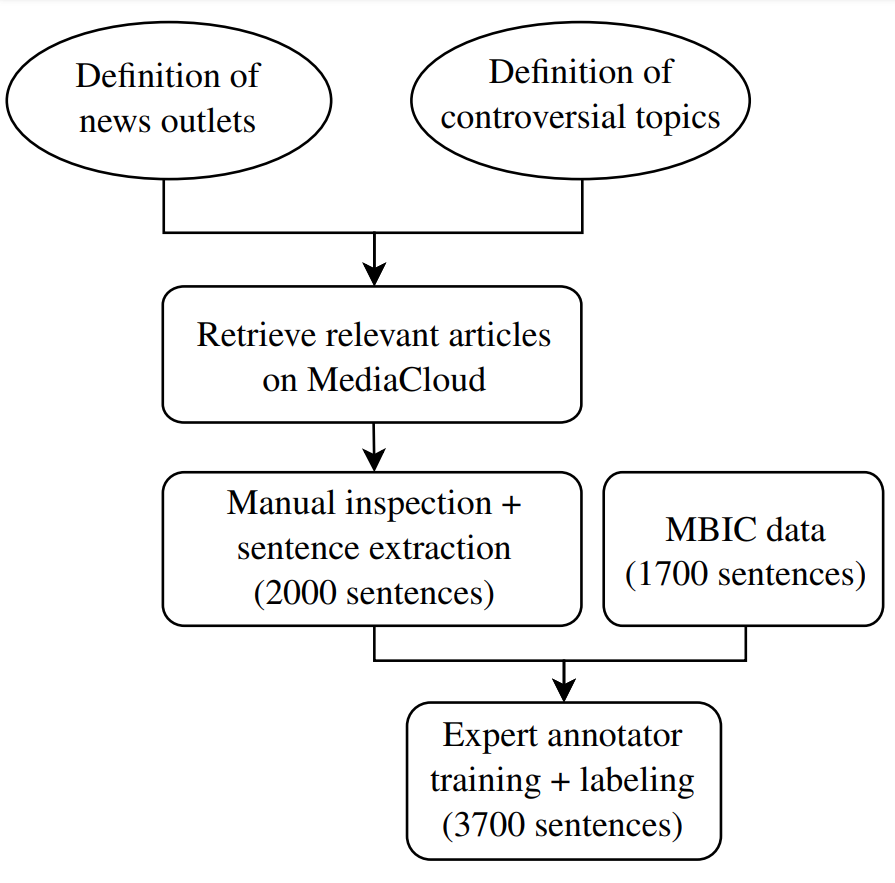
\includegraphics[scale=0.3]{my_modules/multimedia/babe_workflow.png}
  \caption{Data collection and annotation pipeline of \textbf{BABE}, reprinted from \cite{Spinde2021f}}
  \label{fig:babe-data}
\end{figure}



\section{Wikipedia NPOV datasets}\label{wiki-npov}
Due to annotation costs and the overall lack of large-scale datasets in the media bias setting, many researches \cite{pryzant2020automatically,recasens2013linguistic,hube2019neural} used Wikipedia's \Gls{npov} policy\footnote{\url{https://en.wikipedia.org/wiki/Wikipedia:Neutral_point_of_view}} to construct large-scale corpora automatically. 

Wikipedia's NPOV policy is a set of rules which aim to preserve neutrality in Wikipedia articles. Some examples of NPOV principles are:
\begin{itemize}
    \item Avoid stating opinions as facts.
    \item Avoid stating facts as opinions.
    \item Prefer nonjudgmental language.
\end{itemize}

When neutrality is contested, Wikipedia article can be moved to NPOV dispute by tagging it with \{\{NPOV\}\} or \{\{POV\}\}\footnote{Other POV related variations are ofthen used.} template. Debate on specific details of neutrality violations is then initialized among editors and eventually resolved, leading to removal of the tag.

This editorial information can be leveraged to extract parts of the text that violate NPOV and their unbiased counterparts. However, it has been shown \cite{hube2019neural,zhong-etal-2021-wikibias-detecting} that such automatic extraction can suffer from noisy labelling. In some cases \cite{hube2019neural} up to 60\% of data positive points were actually neutral.

Even though these datasets introduce a large amount of samples that are highly related to media bias, they are all sampled from Wikipedia's environment, which can be very different from the news environment. Effect of this domain gap on a training of a model is studied in \ref{experiments} section.




\subsection{Wiki Neutrality Corpus}\label{wiki}
\Gls{wnc} \cite{pryzant2020automatically} is a parallel corpus of 180k pairs of biased and unbiased sentences. For the collection of the data, \ref{wiki-npov} approach was adopted. The authors crawled revisions from 2014 - 2019. Each revision has been processed to check if it contains any variation of \textit{POV} related text in it. This approach yielded 180k pairs such that the sentence before edit is considered biased and the modified/added sentence after edit is considered neutral/unbiased.
    
In addition to WNC, 385k of sentences which have not been changed during the NPOV dispute were extracted as neutral and for word-level classification purposes, a subset of WNC corpus, where only one word is changed in the biased-unbiased pair, were added.




\subsection{CW-HARD}
Hube et al. \cite{hube2019neural} constructed a dataset based on NPOV, where only revisions with one sentence diff were filtered. However, because of the potentially noisy outcome, 5000 sentences were sampled and annotated using crouwdsourcing. Yet, the Krippendorffs Alpha agreement score measured only $\alpha = 0.124$ which is generally considered low. 

After filtering out sentences which annotators labeled with "I dont know" option, the final dataset consists of 1843 statements labeled as biased and 3109 labeled as neutral, a total of 4953 sentences.




\subsection{WikiBias}
This is the latest dataset based on Wikipedia. The authors \cite{zhong-etal-2021-wikibias-detecting} closely follow the approach of WNC \cite{pryzant2020automatically} and extract another parallel wiki corpus of 214k sentences.
To achieve a higher quality corpus, 4099 sentence pairs were randomly sampled and labeled by trained annotators. As a result, introduced \textbf{WikiBias-Manual} dataset consists of 3400 biased and 4798 neutral sentences annotated with high \gls{iaa} score of Cohen's $\kappa = 0.734$

\begin{table}
\begin{ctucolortab}
\begin{tabular}{c|c|c|c}
 \textbf{Dataset} & \textbf{Size} & \textbf{Annotation} & \textbf{Agreement}\\
 \hline
 \textbf{SUBJ} & 10.000 & automatic & -\\ 
 \hline
 \textbf{MPQA} & 15.802 & annotators & high \\
 \hline
 \textbf{BASIL} &  1.727 & annotators & medium \\ 
 \hline
 \textbf{Ukraine Crisis Dataset} & 2.057 & crowdsourcing & low \\ 
 \hline
 \textbf{NFNJ} & 888 & crowdsourcing & low \\
 \hline
 \textbf{BABE} & 3673 & annotators & medium \\
 \hline 
 \textbf{WNC} & 362.990 & automatic & - \\
 \hline
 \textbf{CW-hard} & 4953 & crowdsourcing & low \\
 \hline 
 \textbf{WikiBias} & 8198 & annotators & high \\
 \hline
\end{tabular}
\end{ctucolortab}
\caption{Comparison of all bias related datasets collected}
\label{table:1}
\end{table}



\section{Unused datasets}
 Some datasets focus on a slightly different task, yet still carry potentially useful information. Such data can be useful in a Multi-Task setting \ref{mtl}. To name a few, which are focused on a detection of ideology:
\begin{itemize}
\item \textbf{NewsB} - 
Consists of labels capturing authors political ideology (liberal, conservative) Labeled through distant supervision.
\item \textbf{IBC} - Also focuses on ideology detection, however, it is not publicly available.
\end{itemize}


\section{Summary}
In the previous section, I introduced all resources that are potentially useful for media bias analysis and are publicly available. The overview of all datasets and its properties can be seen in figure \ref{table:1}.

BABE dataset is generally a good benchmark and its translated parallel version will be used for evaluation in this work. Combinations of different datasets merging are studied in \ref{experiments}. Unfortunately a lot of the data suffer from noisy labelling and low \gls{iaa} greatly. Hence, their usability is considerably limited.


\chapter{Czech datasets}
Czech language is a so-called \textbf{low resource language}, which, in the machine learning community, means that, for a particular language, a limited number of datasets of sufficient quality and size is available. Thus, the bias detection task in the Czech environment is complicated. Despite the relatively sufficient number of datasets in English, there is essentially no suitable Czech one.

 In essence, three options are feasible to solve this problem. The most promising way is to annotate a new gold-standard dataset. However, media bias is a non-trivial, complex, and subtle linguistic feature; hence,a lot of effort must be put into annotator training and eventually filtering of implicitly biased annotations.
 
 Another way is to use an automatic approach. \textbf{Allsides}\footnote{\url{https://www.allsides.com/unbiased-balanced-news}}for example, provide annotations on source and article-level with expert annotation quality. However, since I focus on a statement level only, using such data leads to oversimplification and results in a very noisy dataset. Regardless, it can still be used for domain-specific pretraining \cite{Spinde2021f}. Unfortunately, there is no Czech site that would provide \textbf{useful} bias information on neither source nor article level. The server \Gls{nfnz} \footnote{https://www.nfnz.cz/} provides scoring for different news sources. Yet, only a fraction of their scoring is related to the actual linguistic aspect of the writing. Most of the scoring is based on meta-information such as transparency, proper citation, advertisement, etc.
 
 Nonetheless, the automatic creation of a dataset can be done in a convenient way, as described in section \ref{wiki-npov}. Despite the limitation caused by the size of the particular Wikipedia, this approach is suitable for the Czech environment, as the Czech Wikipedia has a comparably large editor base\footnote{ \url{https://en.wikipedia.org/wiki/List_of_Wikipedias}} ranking \#26 in a number of edits worldwide. I took this approach and present a \textbf{new parallel corpus} for bias detection based on Czech Wikipedia \ref{wncs}.
 
 Finally, for low-resource languages, it is reasonable to translate English datasets. As one of my contributions to bias detection in Czech news, I reviewed, collected and translated most of the relevant datasets described in chapter \ref{datasets} using \textbf{DeepL}, and finally processed them into a unified format \ref{processing}.
 
 
 
 
 
\section{Machine Translation}\label{DeepL}
Since the translation of large datasets by human translators would be too costly and, from a time perspective, practically impossible, automatic machine translation systems are used. In recent years, machine translation, like other fields of \Gls{nlp}, has experienced a significant increase in performance due to the rise of the attention mechanism and complex transformer architectures \ref{att_transformers}.

Modern machine translation models use the \textbf{encoder-decoder} where the encoder part distills (encodes) the information from the input sequence, and the decoder part is responsible for decoding this distilled information and mapping it to a sequence in the target language. For more details, see \ref{theory}.

For the translation of the datasets, I chose \textbf{DeepL} translator, which is a purely\footnote{For example Google combines \Gls{nmt} with statistical approaches, other systems incorporate hardcoded rules, etc.} \Gls{nmt} based system which outperforms other translation systems by a large margin.






\section{Processing}\label{processing}
Every dataset has been processed into "sentence,label" format, where $label \in \{0,1\}$ stands for \textbf{unbiased} and \textbf{biased}, respectively. Using this simplified data format makes merging and combining several datasets convenient. All sentences that were originally cased were \textbf{not} lowercased, and during the training of the classifier, the maximum sentence length was set to 128 tokens. No other pre-processing was used.

\section{Translated data}
All translated datasets are listed below. I hope that this collection will serve as a good starting point for future \gls{mb} research in Czech News.

I will share all the listed datasets on HuggingFace\footnote{\url{https://huggingface.co/}} hub.

\begin{itemize}
    \item BABE-CS
    \item Basil-CS
    \item WikiBias-CS
    \item CW-hard-CS
    \item MPQA-CS
    \item NFNJ-CS
    \item SUBJ-CS
    \item UA-crisis-CS
    \item WNC-large-CS\footnote{additional \textit{large} is added to distinguish between large translated WNC and the Czech version of WNC}
\end{itemize}

Together, approximately 400k bias-labeled translated sentences were collected. The distribution of the datasets can be seen in figure \ref{fig:cz_data}. The WNC is not included in the plot because it represents 87\% of all data. 


\begin{figure}
  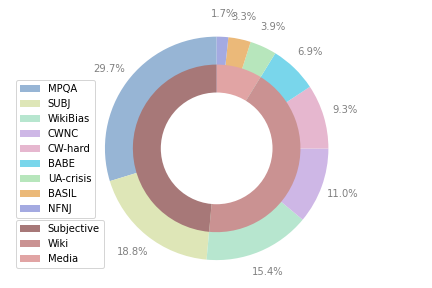
\includegraphics[scale=0.5]{my_modules/multimedia/withoutWNC.png}
  \caption{Dataset distribution in czech collection of data (Without WNC)}
  \label{fig:cz_data}
\end{figure}




\section{Czech Wiki Neutrality Corpus}
Finally, I present two novel parallel corpora extracted directly from Czech Wikipedia. To the best of my knowledge, this is the only original Czech dataset related to media bias detection. The only partially relevant dataset is \textbf{SubLex}\cite{11858/00-097C-0000-0022-FF60-B} which is a subjectivity lexicon focusing mainly on sentiment. However, lexicon-based approaches are nowadays outperformed by neural models.

I followed two main existing approaches, both relying on the extraction of revisions that includes the \{\{NPOV\}\} tag or its variation. The NPOV tag also has its Czech version \Gls{nup}. However, the Czech version is practically not used, and so for the extraction, the English variations were used.





\subsection{CWNC-noisy}
I closely followed the \cite{aleksandrova2019multilingual} approach and used their publicly available script. Firstly, a file with all pages and its complete edit history is downloaded from the wiki dump\footnote{\url{https://dumps.wikimedia.org/cswiki/}}. I used the \textbf{20220201} version. Then, the pages with edits containing one of the NPOV-related tags are filtered, and the process of sentence extraction follows.
This approach yielded 15k sentences; however, it uses a rather trivial assumption that when the NPOV tag is removed, \textbf{all} removed sentences are biased and all added are unbiased. This annotating strategy led to a very noisy dataset, and for this reason, I excluded this dataset from further experiments entirely.


\subsection{CWNC}\label{wncs}
This dataset was created following the \cite{pryzant2020automatically} approach. The process is the same as described in section \ref{wiki-npov}. I used \textbf{20220201} snapshot of Wikipedia dump, which was, at the time of dataset collection, the latest snapshot that included all necessary files.
I used the script publicly available on Github\footnote{\url{https://github.com/rpryzant/neutralizing-bias}},with a few slight modifications so the processing fits the Czech language properties:
\begin{enumerate}
    \item Used Regex was extended to exclude czech words that contain "pov" inside eg. \underline{pov}stání, \underline{pov}lak etc.
    \item All cases has been preserved.
    \item Czech Morphodita tokenizer was used\footnote{\url{https://ufal.mff.cuni.cz/morphodita/users-manual}}
\end{enumerate}
The final dataset consists of:
\begin{itemize}
    \item 3k of \textit{before} and \textit{after} sentence pairs
    \item 1.7k subset where only one word has been changed
    \item 7.5 sentences, where the change was rejected or reversed, implying neutrality of the original sentence.
\end{itemize}

\begin{table}
\makebox[\textwidth][c]{
\begin{tabular}[\textwidth]{|l|}
\hline
\cellcolor{biased_clr} Nizozemsko je známé svým \colorbox{biasedw_clr}{pokrokovým} liberálním postojem vůči psychoaktivním drogám.\\
\cellcolor{unbiased_clr} Nizozemsko je známé svým liberálním postojem vůči psychoaktivním drogám.\\
\hline
\hline
 \cellcolor{biased_clr} Mezi jeho nejznámější a zvlášť populární je jeho hudba ke hrám a filmům, která téměř zlidověla.\\
 \cellcolor{unbiased_clr} Mezi jeho nejznámější a zvlášť populární je jeho hudba k divadelním hrám a filmům, která \\
 \cellcolor{unbiased_clr} v některých případech téměř zlidověla.\\
\hline
\end{tabular}
}
\caption{Example of pairs of biased sentences and their rewritten neutral form}
\label{table:cwnc_example}
\end{table}


In total, 5766 sentences. The neutral corpus, which contains only neutral sentences, is saved for a potential need of oversampling. Two examples of CWNC sentence pairs can be seen in \ref{table:cwnc_example}





\section{Not translated}
Due to a large size of some datasets, I was unable to translate more than one large-scale dataset. For this reason, the NewsB dataset has not been translated.

\chapter{Theoretical background}

\section{Neural Networks }
\section{Attention and transformers}\label{att_transformers}
\section{Transfer learning}
\section{Text classification}
\subsection{Metrics}
\begin{itemize}
    \item F1 \label{f1}
\end{itemize}
\section{Multi-Task learning}


\chapter{Experiments}\label{experiments}
In this section I present experiments on text classification over colelcted datasets. Main target dataset for evaluations is BABE, because of its high quality and properties.

Because of novelty of CWNC I also perform evaluation on this dataset.
I follow the current standard approaches and use pretrained transformers for further pretraining and fine-tuning. One possibility is to use multilingual models, which are trained on set of languages to capture general language properties. In recent years, there have also purely czech models emerged.
\subsection{Czech models}
\begin{itemize}
    \item RobeCZECH
    \item Czert
    \item FERNET-C5
    \item FERNET-News
\end{itemize}


\subsection{Multi-lingual models}
\begin{itemize}
    \item SlavicBert
    \item mBERT
\end{itemize}


 15\% of BABE data has been saved for final evaluation. Steps are as follows:
 \begin{itemize}
     \item BASELINE:
	5-CV plain model finetuning on BABE (could be split to train validation but we dont have that many data)
	\item HYPERPARAM-TUNING:
	5-CV model tuning parameters (grid search) on BABE
	\item DATA-COMBINATIONS:
	5-CV model with tuned hyperparams with varying combinations of data on BABE
	\item EVALUATION:
	pick the best model, train it with params and early stopping, and run it on - BABE test set 
										       - CWNC test set
	early stopping only on final training! Because the authors essentially made early stopping on "testing set" + it is not recommended to use early stopping in cross validation
 \end{itemize}
 
 
 
 
 
All training has been done on a single GPU on RCI cluster.
 \section{Baseline setup}
 As a baseline, I finetuned all Czech models listed above on BABE and evaluated them using 5-fold stratified cross validation. Hyperparameters were the same as used by authors \cite{Spinde2021MBIC}. However, the authors used 10 epochs and early stopping, together with cross validation and used the validation split inside CV to early stop, which is not ideal since the split should be used only for evalaution. That way the model can "see" the data before evaluation, hence I did not use early stopping with CV at all and fixed number of epochs on 3, as authors of BERT \cite{devlin2019bert} suggest. 
 All other hyperaparemeters remained unchanged. Adam optimizer is used with learning reate $5e-5$
 
 
 
 
 
 \section{Hyperparameter tuning}
 To get the most out of the language models, I decided to tune the hyperparameters via Bayesian Optimization framework. Because a complexity of searching for optimal hyperparameters grows exponentially with number of items, it is reasonable to not try every combination. Bayesian optimization limits this search space by using Bayes theorem.
 
 
 
 
 \section{Combining Datasets}
 Here i can combine datasets.
 \subsection{Pretraining on English WNC}
 \subsection{Subjectivity pretraining}
 \subsection{Media Bias Pretraining}
 \subsection{Combining all datasets together Without WNC}

 
 
 
 
\section{Inference on Czech News Samples}
\begin{itemize}
    \item Analysis and statistics
    \item Few words Article level
\end{itemize}

%\section{LIME analysis and demo}

\section{Multi-Task learning approach}\label{mtl}

\chapter{Conclusion}
\section{Future work}
\section{Ethical concerns}




\printindex

\bibliographystyle{ieeetr}
\bibliography{my_modules/citation}
\printglossary
\appendix
\chapter{Gender classification results}\label{gender_results}

\begin{figure}[H]
\makebox[\textwidth][c]{
  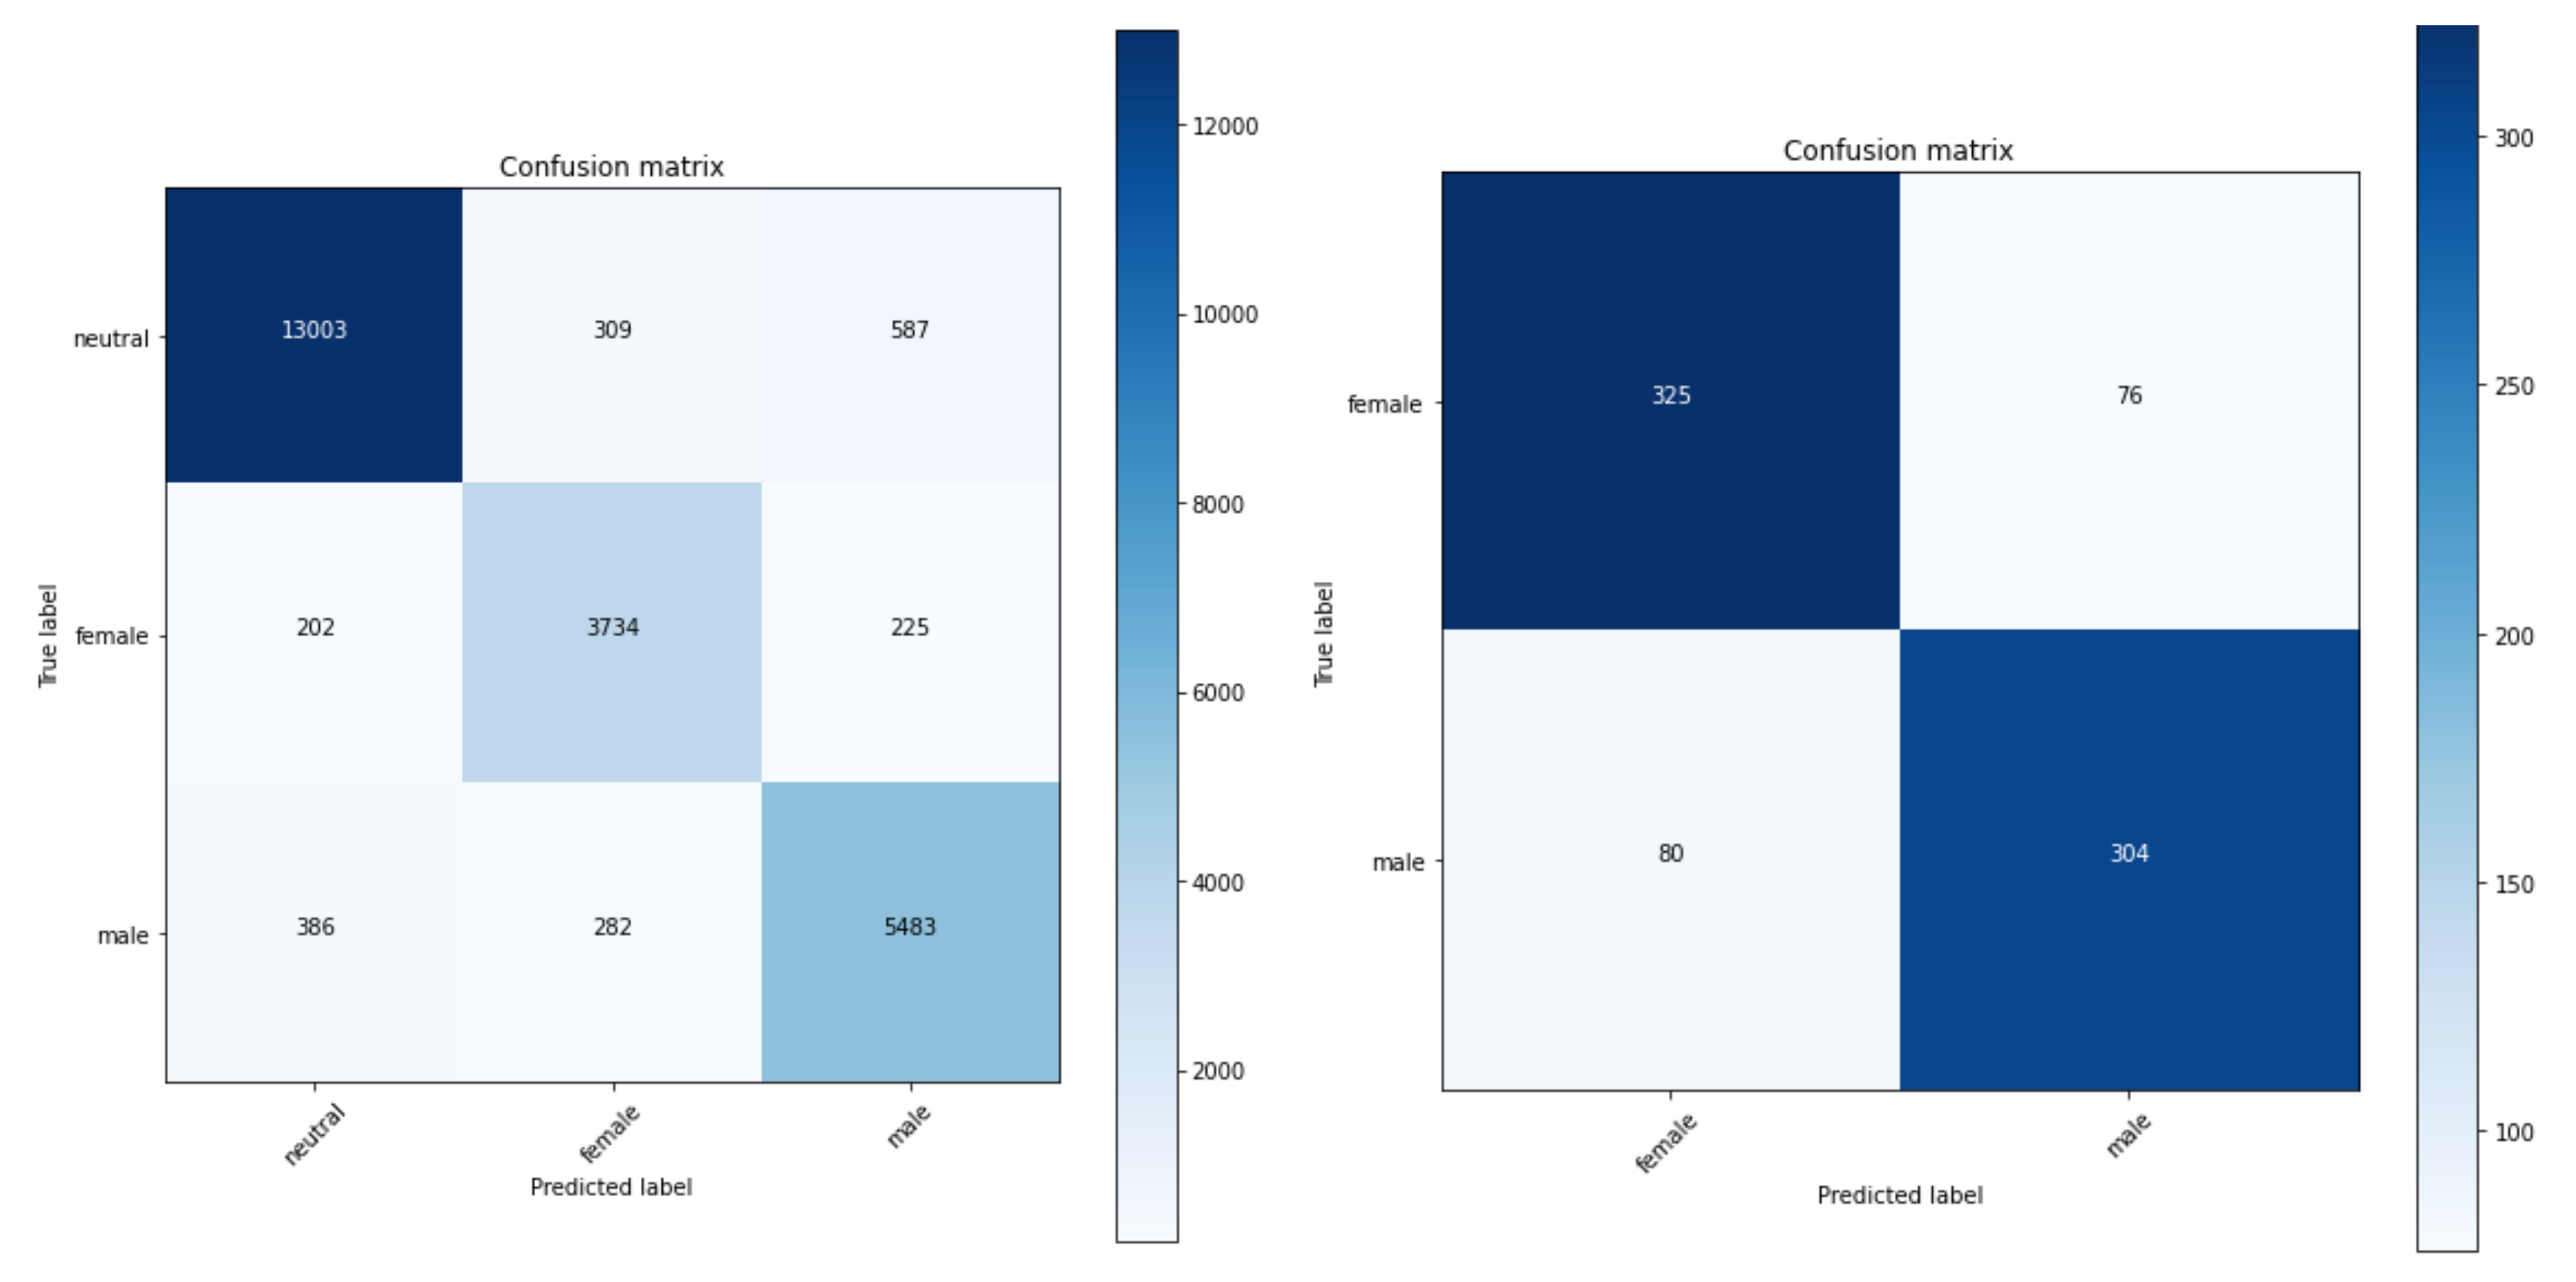
\includegraphics[scale=0.52]{my_modules/multimedia/cfmats.png}
  \caption{Confusion matrices of gender classifier on test sets. On the left on large scale validation dataset. On the right on a gold-label small test set.}
  \label{fig:gender_cfmats}
  }
\end{figure}


\begin{figure}[H]
\makebox[\textwidth][c]{
  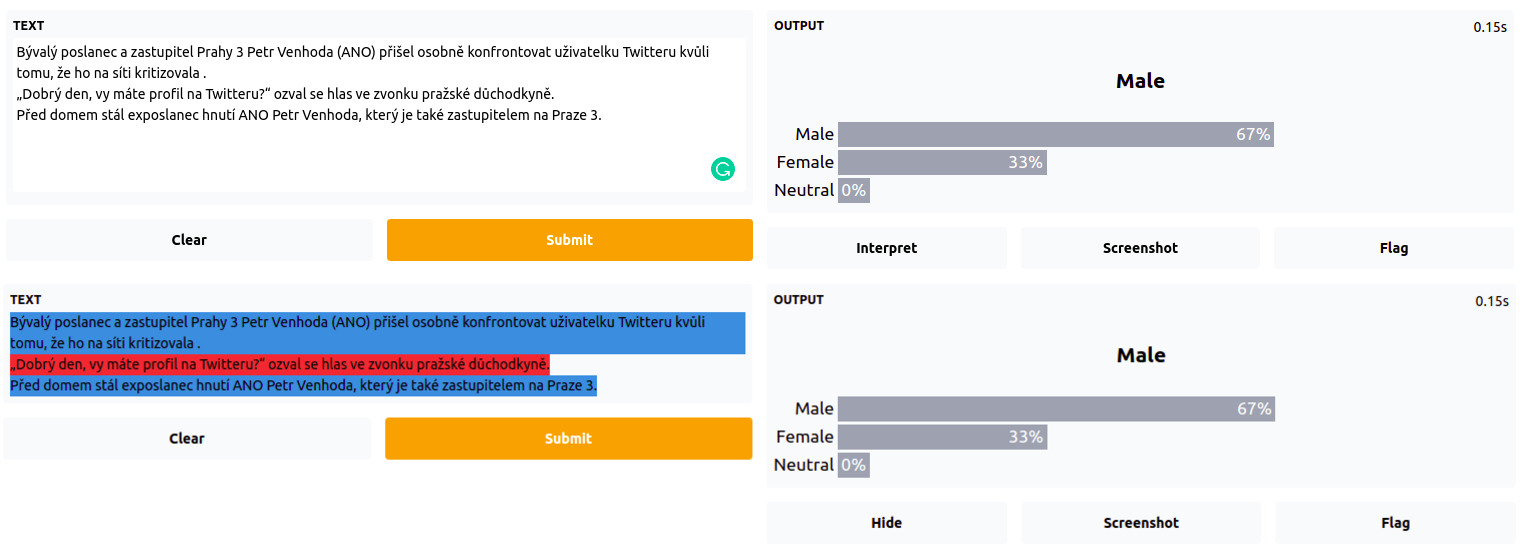
\includegraphics[scale=0.3]{my_modules/multimedia/gender_classifier.jpg}
  \caption{Example of the gender bias classification.}
  \label{fig:gender_classification}
  }
\end{figure}





\end{document}